\documentclass[12pt]{report}
\usepackage{./mystyle}
\usepackage{./slashbox}
\newlist{todolist}{itemize}{2}
\setlist[todolist]{label=$\square$}
\usepackage{pifont}
\newcommand{\cmark}{\ding{51}}%
\newcommand{\xmark}{\ding{55}}%
\newcommand{\done}{\rlap{$\square$}{\raisebox{1pt}{\large\hspace{2.5pt}\cmark}}%
\hspace{-2.5pt}}
\newcommand{\wontfix}{\rlap{$\square$}{\large\hspace{1pt}\xmark}}
\begin{document}
\newcommand{\HRule}{\rule{\linewidth}{0.5mm}}

\begin{titlepage}

\centering
	
\includegraphics[width=0.2\textwidth]{./title/logohse.png}\par\vspace{1cm}
	{\scshape \LARGE Higher School of Economics \\ \small(National Research University)\par}
	{\scshape \Large Faculty of Computer Science\par}
	\vspace{3cm}
	{\scshape\Large Home Assignment \par \Large{Course: ``Modern Methods of Data Analysis''}\par}
%	\vspace{1cm}
    \HRule \\[0.5cm]
    { \Large \bfseries Medium Articles Analysis}\\[0.2cm] % Title of your document
    \HRule
	\vspace{3.5cm}
	\begin{flushright}
	Student: Ryabykin Alexey \\
	Professor: Ignatov Dmitriy Igorevich
	\\
	Grade: \underline{\hspace{0.2cm}}
    \end{flushright}
    \vfill

	{\large Moscow, 2022}
\end{titlepage}
\boldmath
\tableofcontents
\newpage
\pagestyle{fancy}

\fancyhead[L]{LazyFCA}
\fancyhead[C]{\currentname}
\fancyhead[R]{Alexey Ryabykin}

\section{Task description}
This homework serves as an entry point for students into the data science world.
So it introduces students to three main topics:

\begin{enumerate*}
  \item Typical machine learning project:
  \par 
  The pipeline of loading a dataset, feature engineering, designing a new predictive algorithm, results comparison;
  \item Lazy learning:
  \par Predicting labels for small or rapidly changing data;
  \item Rule-learning (on part with FCA):
  \par 
  Viewing data as binary descriptions of objects (instead of points in a space of real numbers).
\end{enumerate*}

{\Large ToDo list}:
\begin{todolist}
  \item[\wontfix] Find a dataset for binary classification;
  \item[\wontfix] Describe scaling (binarization) strategy for the dataset features;
  \item[\wontfix] Describe quality measure best suited for the dataset'
  \item[\wontfix] Adapt the pipeline from \emph{lazyfca.ipynb} to your task;
  \item[\wontfix] Improve the baseline algorithm: 
      \begin{todolist}
          \item[\wontfix] Achieve better asymptotic complexity;
          \item[\wontfix] Improve the rruntime of examples comparison;
          \item[\wontfix] Rewrite the intersections of sets into the intersection of the corresponding bitmasks;
          \item[\wontfix] Modify the algorithm to achieve better qualtiy of predictions.
      \end{todolist}
      \item[\wontfix] Compare the proposed algorithm with at least 3 popular rule-based models;
      \item[\wontfix] Test the proposed algorithm on more datasets (at least 3 others);
      \item Incorporate pattern structure into the pipeline to avoid scaling (binarization).
\end{todolist}


\section{The chosen datasets}
I have chosen three datasets to check the initial algorithm and my proposed one perfomances. They all belongs to UCI Machine Learning Repository. The first one is Car dataset (1728 instances). You can watch the description of variables below:
\begin{itemize}
  \item target: car acceptabiltiy;
  \par It is not a binary feature (possible values: ``unacc'', ``acc'', ``good'', ``v-good''). But two classes cover 92\% of the dataset. I have merely dropped the least classes and obtained binary classification task. But it is still very bad balanced dataset. That is why the preffered metric to estimate the algorithm perfomances had been chosen f1 score.
  \item buying: buying price;
  \par 
  Possible values: ``v-high", ``high", ``med", ``low''. Applying the one-hot encoding is the best strategy to make binarization to this feature;
  \item maint: price of the maintenance;
  \par Possible values: ``v-high", ``high", ``med", ``low''. The same strategy for binarization as for the previous feature.
  \item doors: number of doors;
  \par Possible values: ``2'', ``3'', ``4'', ``5more''. The same strategy.
  \item persons: capacity in terms of persons to carry;
  \par Possible values: ``2'', ``3'', ``4more''. One-hot encoding.
  \item lug\_boot: the size of luggage\ boot;
  \par Possible values: ``small'', ``med'', ``big''.
  \item safety: estimated safety of the car;
  \par Possible values: ``low'', ``med'', ``high''.
\end{itemize}
The second dataset is the Mushrooms dataset. The description of the variables below:
\begin{itemize}
  \item cap-shape: \par bell = b, conical = c, convex = x, flat = f,
  knobbed = k, sunken = s;
  \item cap-surface: \par fibrous = f, grooves = g, scaly = y, smooth = s;
  \item cap-color: \par brown = n, buff = b, cinnamon = c, gray = g, green = r, pink = p, purple = u, red = e, white = w, yellow = y;
  \item bruises?:         \par bruises = t, no = f;
  \item odor:  \par almond = a, anise = l, creosote = c,fishy = y, foul = f,
  musty = m, none = n, pungent = p, spicy = s;
  \item gill-attachment:  \par attached = a, descending = d, free = f, notched = n;
  \item gill-spacing:   \par close = c, crowded = w, distant = d;itemize
  \item gill-size:     \par broad = b, narrow = n;
  \item gill-color:    \par black = k, brown = n, buff = b, chocolate = h, gray = g, 
  green = r, orange = o, pink = p, purple = u, red = e, 
  white = w, yellow = y;
  \item stalk-shape:   \par            enlarging = e, tapering = t;
  \item stalk-root:     \par           bulbous = b, club = c, cup = u, equal = e, 
  rhizomorphs = z, rooted = r, missing = ?;
  \item stalk-surface-above-ring:\par  fibrous = f, scaly = y, silky = k, smooth = s;
  \item stalk-surface-below-ring:\par  fibrous = f, scaly = y, silky = k, smooth = s;
  \item stalk-color-above-ring:\par    brown = n, buff = b, cinnamon = c, gray = g, orange = o, 
  pink = p, red = e, white = w, yellow = y;
  \item stalk-color-below-ring: \par   brown = n, buff = b, cinnamon = c, gray = g, orange = o, 
  pink = p, red = e, white = w, yellow = y;
  \item veil-type:     \par            partial = p, universal = u;
  \item veil-color:    \par            brown = n, orange = o, white = w, yellow = y;
  \item ring-number:    \par           none = n, one = o, two = t;
  \item ring-type:      \par           cobwebby = c, evanescent = e, flaring = f, large = l, 
  none = n, pendant = p, sheathing = s, zone = z;
  \item spore-print-color:  \par       black = k, brown = n, buff = b, chocolate = h, green = r, 
  orange = o, purple = u, white = w, yellow = y;
  \item population:      \par          abundant = a, clustered = c, numerous = n, 
  scattered = s, several = v, solitary = y;
  \item habitat:       \par            grasses = g, leaves = l, meadows = m, paths = p, 
  urban = u, waste = w, woods = d.
\end{itemize}
The last dataset is the United States Congressional Voting Records Database. The values description is presented below:
\begin{multicols}{2}
  \begin{itemize}
    \item target: 2 (democrat, republican)
    \item handicapped-infants: 2 (y,n)
    \item water-project-cost-sharing: 2 (y,n)
    \item adoption-of-the-budget-resolution: 2 (y,n)
    \item physician-fee-freeze: 2 (y,n)
    \item el-salvador-aid: 2 (y,n)
    \item religious-groups-in-schools: 2 (y,n)
    \item anti-satellite-test-ban: 2 (y,n)
    \item aid-to-nicaraguan-contras: 2 (y,n)
    \item mx-missile: 2 (y,n)
    \item immigration: 2 (y,n)
    \item synfuels-corporation-cutback: 2 (y,n)
    \item education-spending: 2 (y,n)
    \item superfund-right-to-sue: 2 (y,n)
    \item crime: 2 (y,n)
    \item duty-free-exports: 2 (y,n)
    \item export-administration-act-south-africa: 2 (y,n)
  \end{itemize}
\end{multicols}

\section{Initial algorithm}
The following algorithm is used in the homework as a baseline algorithm for lazy FCA-based classification. And it is called "Generators framework".
\subsection*{Description}
Assume that we want to make a prediction for description $x \subseteq M$ given the set of training examples \mbox{$X_{\text{train}} \subseteq 2^M$} and the labels $y_x \in \left\{\text{False}, \text{True}\right\}$, corresponding to each $x \in X_{\text{train}}$.

\par 
First, we split all examples $X_{\text{train}}$ to positive $X_{\text{pos}}$ and negative $X_{\text{neg}}$ examples:
\[
  X_{\text{pos}} = \left\{ x \in X_{\text{train}}\ | \ y_x \text{ is True}\right\}, \hspace*{0.5cm} X_{\text{neg}} = X \backslash X_{\text{pos}}.
\]
To classify the description $x$ we follow the procedure:
\begin{enumerate}
  \item Count the number of counterexamples for positive examples:
  \par For each positive example $x_{\text{pos}} \in X_{\text{pos}}$ we compute  the intersection $x \cap x_{\text{pos}}$. Then, we count the counterexamples for this intersection, that is the number of negative examples $x_{\text{neg}} \in X_{\text{neg}}$ containing intersection  $x\cap x_{\text{pos}}$;
  \item Dually, count the number of counterexamples for negative examples. 
\end{enumerate}
Finally, we compare the average number of counterexamples for positive and negative examples. We classify  as being positive if the number of counterexamples for positive examples is smaller the one for negative examples.
\subsection*{Results}
\par 
The table with results and graphics of scores and time information are presented below:
\begin{table}[H]
  \centering
  \begin{tabular}{|c|c|c|c|c|}
    \hline
    \backslashbox{Dataset}{Result}                                                  & accuracy & f1 score & time         & \begin{tabular}[c]{@{}c@{}}time\\ (fixed train)\end{tabular} \\ \hline
    Car                                                       & 0.78     & 0.178    & 37.3 s       & 839 ms                                                       \\ \hline
    Mushrooms                                                 & 0.93     & 0.87     & 2h 23min 44s & 3 min 13 s                                                   \\ \hline
    \begin{tabular}[c]{@{}c@{}}Congress\\ voting\end{tabular} & 0.6      & 0.46     & 303 ms       & 202 ms                                                       \\ \hline
    \end{tabular}
  \caption{Main results for the initial algorithm}
  \end{table}
  Results for the Car dataset are presented on the Figure \ref{fig:car_initial}
  \begin{figure}[H]
    \centering
    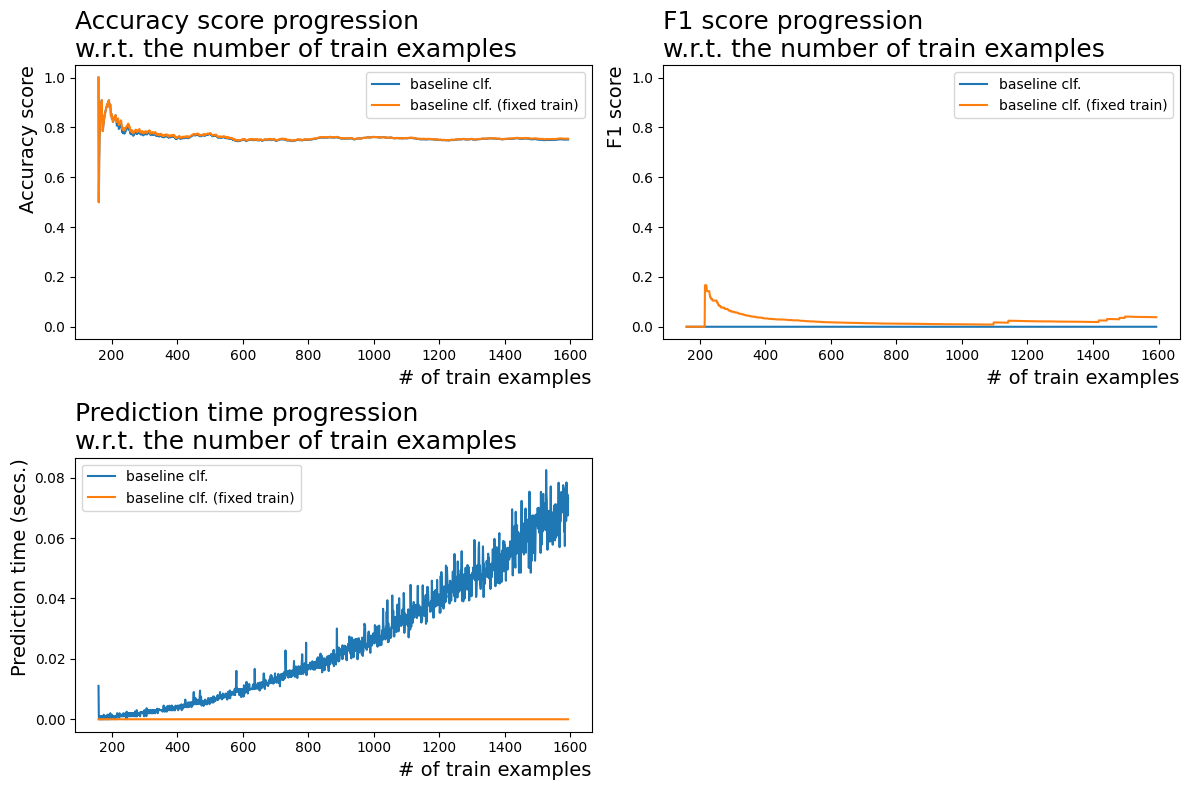
\includegraphics[scale=0.5]{./images/Classifier_comparison_initial_algo_car.png}
    \caption{Results for Car dataset (initial algorithm)}
    \label{fig:car_initial}
  \end{figure}
  You can see on the Figure \ref{fig:mushrooms_initial} the results of the initial algorithm applied to the Mushrooms dataset.
  \begin{figure}[H]
    \centering
    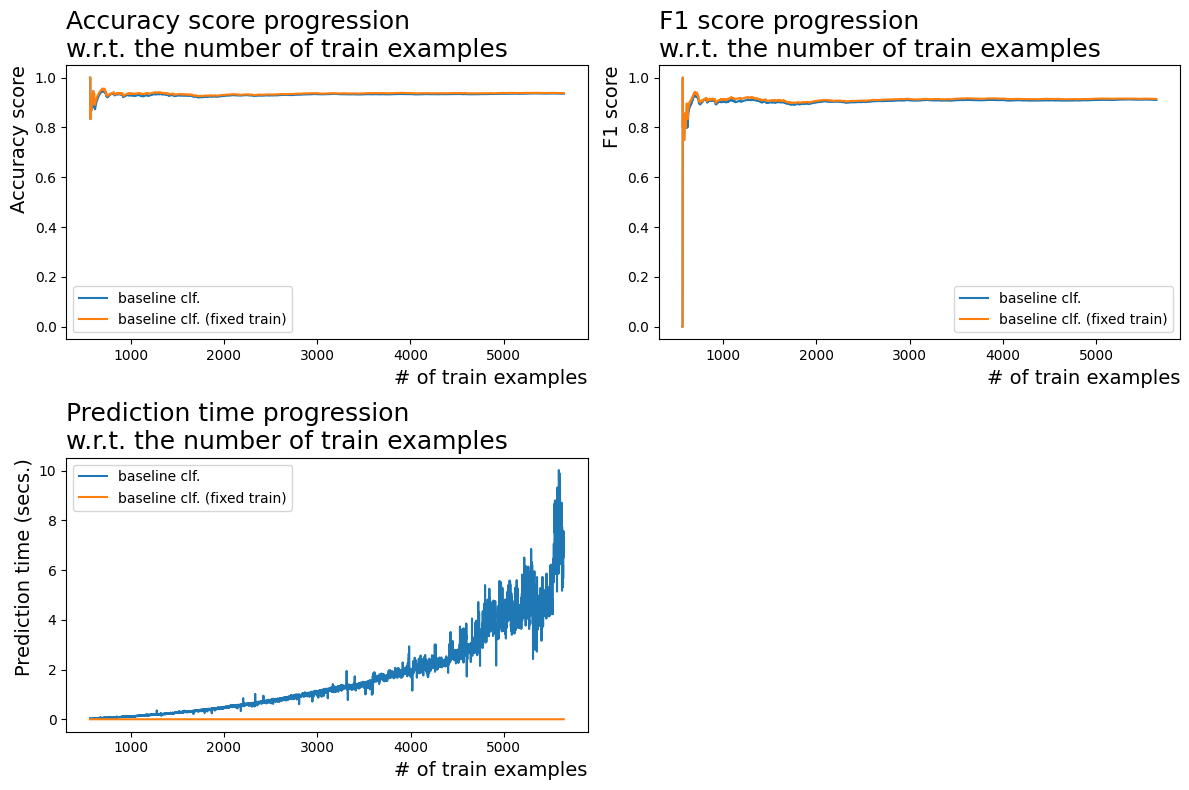
\includegraphics[scale=0.5]{./images/Classifier_comparison_initial_algo_mushrooms.png}
    \caption{Results for Mushrooms dataset (initial algorithm)}
    \label{fig:mushrooms_initial}
  \end{figure}
  The Figure \ref{fig:congress_initial} contains the results of the initial algorithm appication to the Congress Voting dataset. 
  \begin{figure}[H]
    \centering
    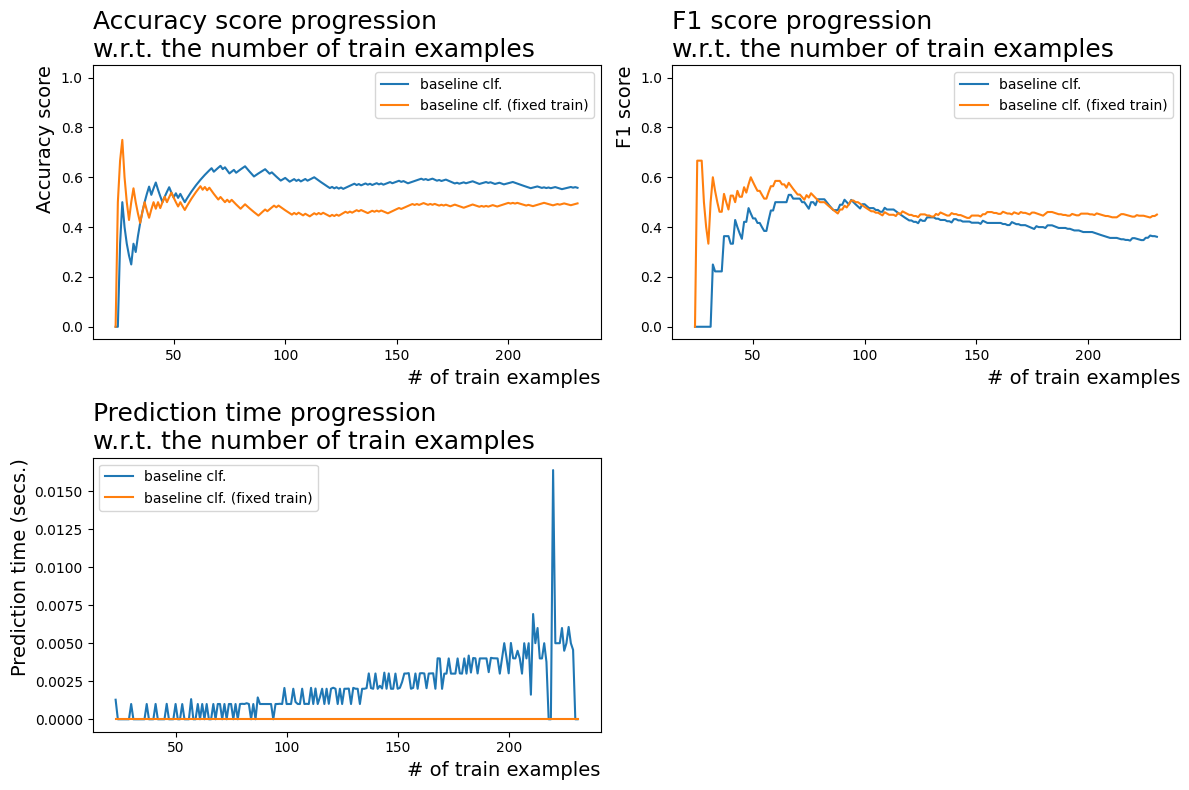
\includegraphics[scale=0.5]{./images/Classifier_comparison_initial_algo_congress.png}
    \caption{Results for Congress Voting dataset (initial algorithm)}
    \label{fig:congress_initial}
  \end{figure}
\section{Proposed improvements and comparisons}
\par 
The core idea is the same as for the initial algorithm. But the chosen path to calculate the intersections is different with the previous one. The procedure can be expressed in terms of matrix multiplication of bitmasks that had been obtained after binarization. The proposed code you can see below:
\begin{lstlisting}[language=Python, caption=Python code]
  def predict_with_generators(
    x: set, X_train: List[set], Y_train: List[bool],
    min_cardinality: int = 1
  ) -> bool:
    X_pos = np.array(X_train[np.array(Y_train, dtype=bool)], dtype=int)
    X_neg = np.array(X_train[~np.array(Y_train, dtype=bool)], dtype=int)

    idxs = X_pos @ x >= min_cardinality
    n_counters_pos = ((X_neg @ (X_pos & x)[idxs, :].T) == (X_pos @ x)[idxs]).sum()

    idxs = X_neg @ x >= min_cardinality
    n_counters_neg = ((X_pos @ (X_neg & x)[idxs, :].T) == (X_neg @ x)[idxs]).sum()

    perc_counters_pos = n_counters_pos / (n_counters_neg + n_counters_pos)
    perc_counters_neg = n_counters_neg / (n_counters_pos + n_counters_neg)
    prediction = perc_counters_pos < perc_counters_neg
    return prediction
\end{lstlisting}

Also, there is some bad influence of proposed in the initial algorithm normalization of counts of counterexamples. In case of bad balanced target values the prediction of the algorithm can be exclusively in the direction of the class, which is larger. I removed the normalization; it improved the quality of the selected datasets. However, on the tic-tac-toe dataset from the baseline, the quality dropped slightly. It can be concluded that normalization is useful, but it should be different. The logic here is that, for example, with 20\% of negative objects in the training sample, finding a negative counterexample is more valuable than a positive one. This must be taken into account.
\begin{table}[H]
  \centering
  \begin{tabular}{|l|c|c|c|c|}
  \hline
  \backslashbox{Dataset}{Result}   & accuracy & f1 score & time   & \begin{tabular}[c]{@{}c@{}}time\\ (fixed train)\end{tabular} \\ \hline
  Car Dataset      & 0.78 & 0.78 & 8.97 s & 563 ms \\ \hline
  Mushrooms & 0.93 & 0.91  & 29 min & 43 s   \\ \hline
  \begin{tabular}[l]{@{}l@{}}Congress\\voting\end{tabular} & 0.92      & 0.9     & 120 ms & 58 ms                                                        \\ \hline
  \end{tabular}
  \caption{Main results for the proposed algorithm}
  \end{table}
  Results for the Car dataset are presented on the Figure \ref{fig:car_improved}
  \begin{figure}[H]
    \centering
    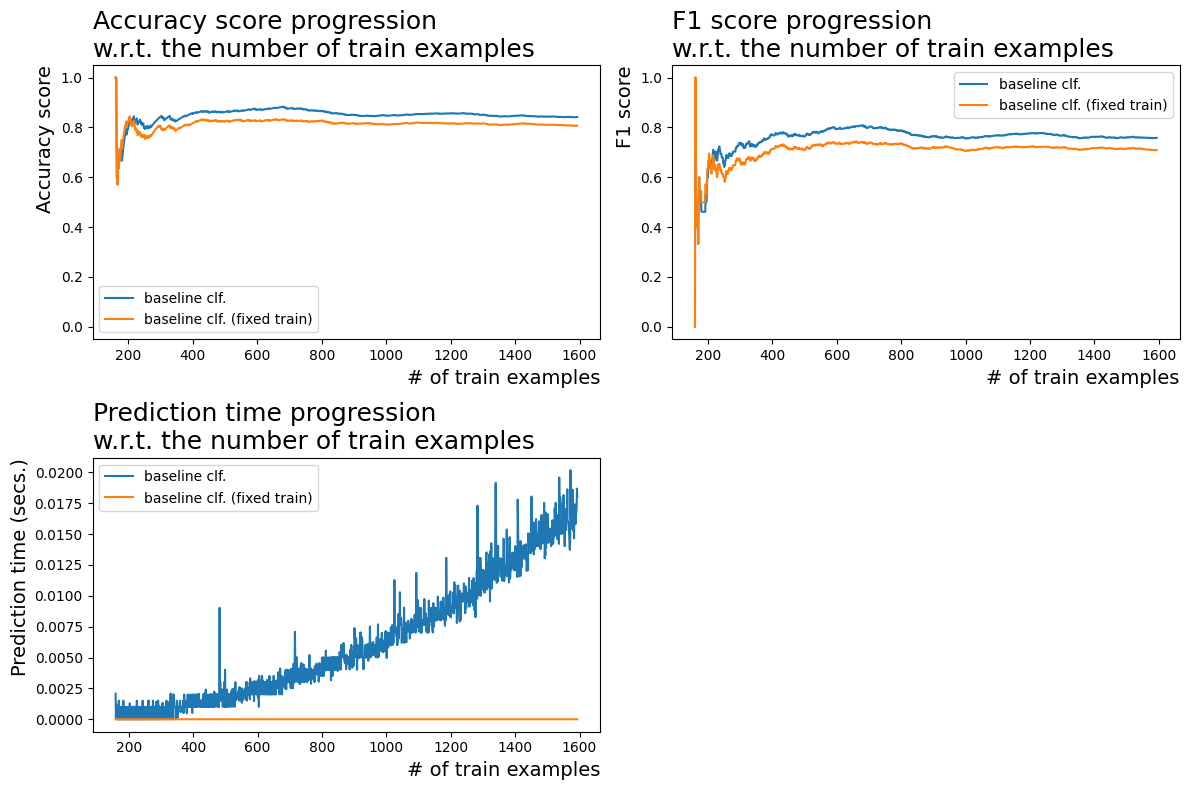
\includegraphics[scale=0.5]{./images/Classifier_comparison_improved_algo_car.png}
    \caption{Results for Car dataset (improved algorithm)}
    \label{fig:car_improved}
  \end{figure}
  You can see on the Figure \ref{fig:mushrooms_improved} the results of the improved algorithm applied to the Mushrooms dataset.
\par
  Let's compare it with the initial algorithm. So, for the Car dataset you can see difference in the Table \ref{table:diff_car}
  \begin{table}[H]
    \centering
    \begin{tabular}{|l|l|l|l|l|}
    \hline
    \backslashbox{CLF}{Result}  & accuracy & f1 score & time  & \begin{tabular}[c]{@{}l@{}}time \\ (fixed train)\end{tabular} \\ \hline
    \begin{tabular}[c]{@{}l@{}}Initial\\ algorithm\end{tabular}   & 0.78     & 0.178    & 37.3s & 839ms                                                         \\ \hline
    \begin{tabular}[c]{@{}l@{}}Proposed \\ algorithm\end{tabular} & 0.78     & 0.78     & 8.97s & 563ms                                                         \\ \hline
    \end{tabular}
    \caption{Comparison of two algorithms on the Car Dataset}
    \label{table:diff_car}
    \end{table}
    \begin{figure}[H]
      \centering
      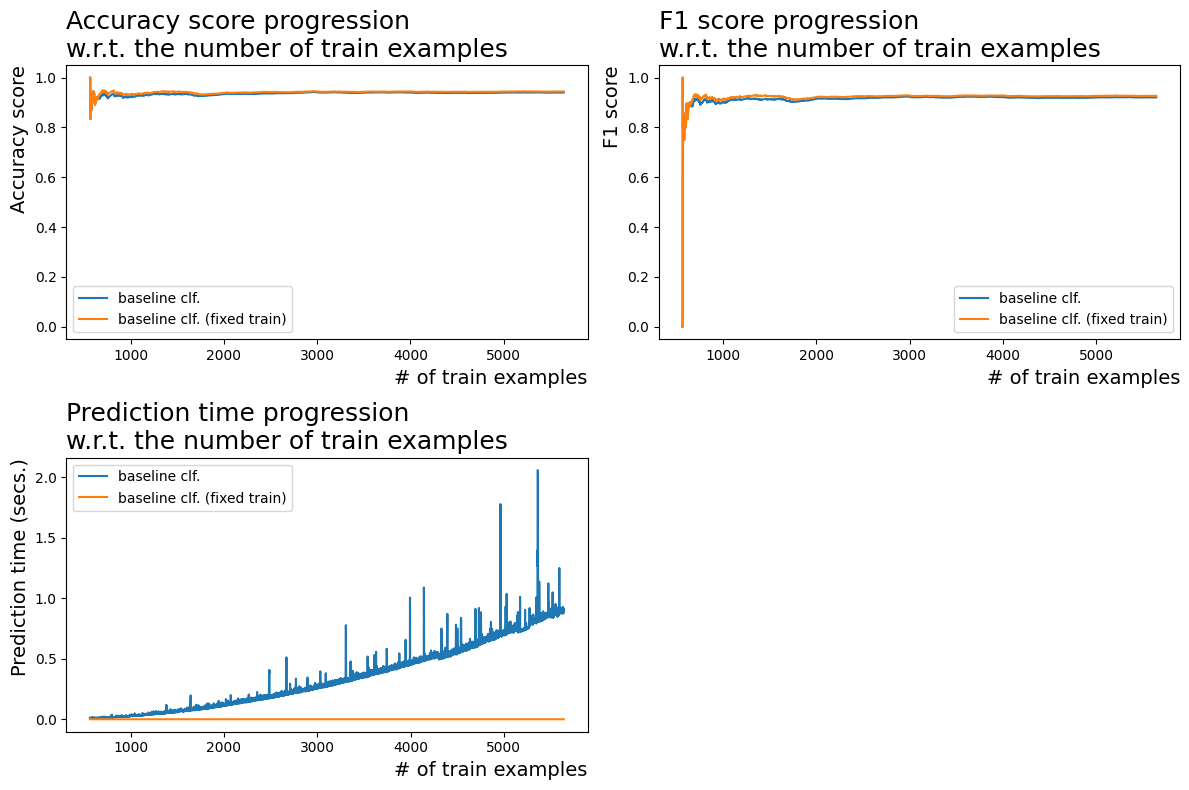
\includegraphics[scale=0.5]{./images/Classifier_comparison_improved_algo_mushrooms.png}
      \caption{Results for Mushrooms dataset (improved algorithm)}
      \label{fig:mushrooms_improved}
    \end{figure}

    Comparison with the initial algorithm is presented below:
    \begin{table}[H]
      \centering
      \begin{tabular}{|l|l|l|l|l|}
      \hline
      \backslashbox{CLF}{Result}                                                          & accuracy & f1 score & time         & \begin{tabular}[c]{@{}l@{}}time \\ (fixed train)\end{tabular} \\ \hline
      \begin{tabular}[c]{@{}l@{}}Initial\\ algorithm\end{tabular}   & 0.93     & 0.9      & 2h 23min 44s & 3min 13s                                                      \\ \hline
      \begin{tabular}[c]{@{}l@{}}Proposed \\ algorithm\end{tabular} & 0.93     & 0.91     & 29min 6s     & 43.5s                                                         \\ \hline
      \end{tabular}
      \end{table}
    The Figure \ref{fig:congress_improved} contains the results of the improved algorithm application to the Congress Voting dataset.
    \par
    Compartison with the initial algorithm is presented below:
    \begin{table}[H]
      \centering
      \begin{tabular}{|l|l|l|l|l|}
      \hline
      \backslashbox{CLF}{Result}a                                                           & accuracy & f1 score & time  & \begin{tabular}[c]{@{}l@{}}time \\ (fixed train)\end{tabular} \\ \hline
      \begin{tabular}[c]{@{}l@{}}Initial\\ algorithm\end{tabular}   & 0.93     & 0.9      & 443ms & 17ms                                                          \\ \hline
      \begin{tabular}[c]{@{}l@{}}Proposed \\ algorithm\end{tabular} & 0.93     & 0.91     & 120ms & 15.6ms                                                        \\ \hline
      \end{tabular}
      \end{table}
    \begin{figure}[H]
      \centering
      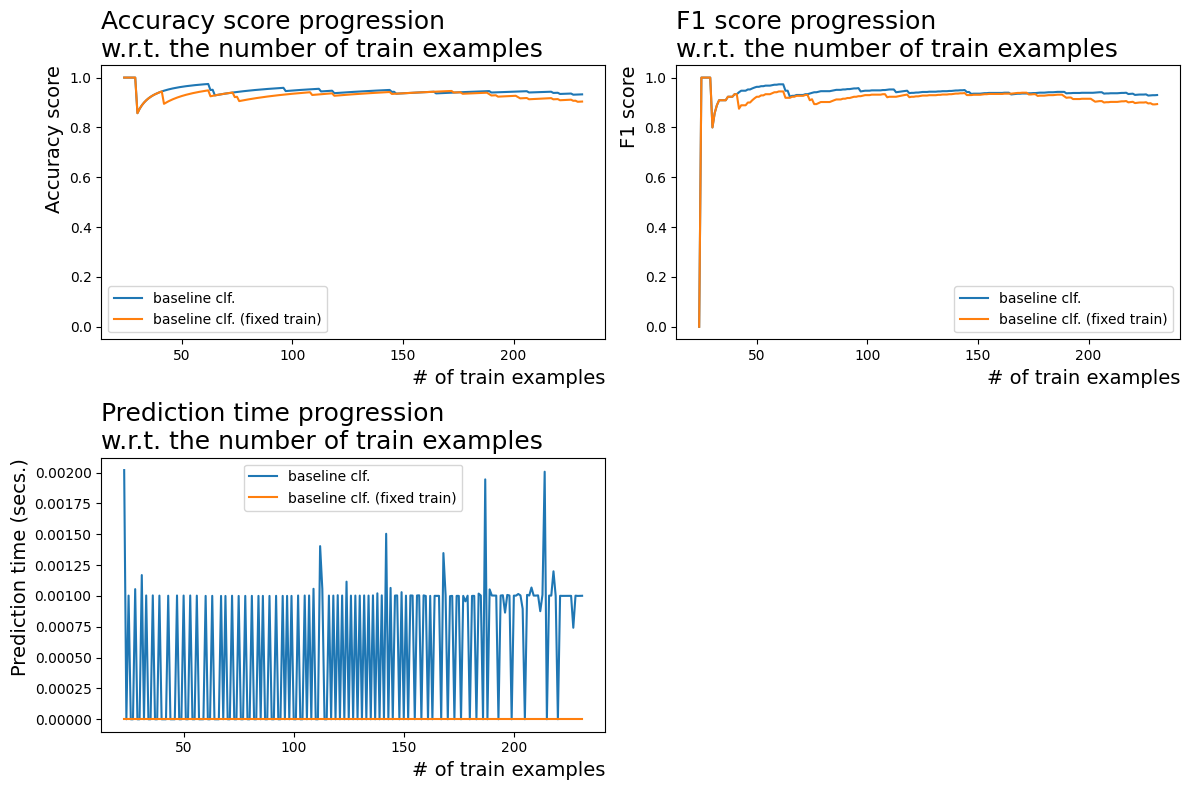
\includegraphics[scale=0.45]{./images/Classifier_comparison_improved_algo_congress.png}
      \caption{Results for Congress Voting dataset (improved algorithm)}
      \label{fig:congress_improved}
    \end{figure}
\section{Comparison with other rule-based models}

\par
The chosen models to compare initial algorithm and algorithm with proposed improvements:
\begin{enumerate}
  \item CatBoostClassifier;
  \item XGBRFClassifier;
  \item LGBMClassifier;
  \item DecisionTreeClassifier;
  \item RandomForestClassifier.
\end{enumerate}
\begin{table}[H]
  \centering
  \begin{tabular}{|l|c|c|c|c|c|c|c|}
    \hline
    \backslashbox{Data}{CLF}                                                                     & \begin{tabular}[c]{@{}l@{}}CatBoost\\ Classifier\end{tabular} & \begin{tabular}[c]{@{}l@{}}DecisionTree\\ Classifier\end{tabular} & \begin{tabular}[c]{@{}l@{}}RandomForest\\ Classifier\end{tabular} & \begin{tabular}[c]{@{}l@{}}XGBRF\\ Classifier\end{tabular} & \begin{tabular}[c]{@{}l@{}}LGBM\\ Classifier\end{tabular} & \begin{tabular}[c]{@{}l@{}}Initial \\ algorithm\end{tabular} & \begin{tabular}[c]{@{}l@{}}Improved \\ algorithm\end{tabular} \\ \hline
    \begin{tabular}[c]{@{}l@{}}Dataset \\ Car\end{tabular}                &       0.958         &       0.816          &       0.743              &    0.796                                                        &   0.813                                                        &   0.78                                                           & 0.78                                                              \\ \hline
    \begin{tabular}[c]{@{}l@{}}Dataset \\ Mushrooms\end{tabular}          &              1                                                 &     0.926                                                              & 0.917                                                                   &      0.932                                                      &  0.927                                                         &  0.93                                                            &             0.93                                                  \\ \hline
    \begin{tabular}[c]{@{}l@{}}Dataset \\ Congress \\ Voting\end{tabular} &                    0.952                                           &       0.966                                                            & 0.961                                                                  &    0.971                                                        &  0.957                                                         &  0.7                                                            &   0.92                                                            \\ \hline
    \end{tabular}
    \caption{Average accuracy scores through cross-validation for the chosen models}
  \end{table}

  \begin{table}[H]
    \centering
  \begin{tabular}{|l|c|c|c|c|c|c|c|}
    \hline
    \backslashbox{Data}{CLF}                                                                     & \begin{tabular}[c]{@{}l@{}}CatBoost\\ Classifier\end{tabular} & \begin{tabular}[c]{@{}l@{}}DecisionTree\\ Classifier\end{tabular} & \begin{tabular}[c]{@{}l@{}}RandomForest\\ Classifier\end{tabular} & \begin{tabular}[c]{@{}l@{}}XGBRF\\ Classifier\end{tabular} & \begin{tabular}[c]{@{}l@{}}LGBM\\ Classifier\end{tabular} & \begin{tabular}[c]{@{}l@{}}Initial \\ algorithm\end{tabular} & \begin{tabular}[c]{@{}l@{}}Improved \\ algorithm\end{tabular} \\ \hline
    \begin{tabular}[c]{@{}l@{}}Dataset \\ Car\end{tabular}                &                                                              0.921 &        0.838      &        0.829           &      0.844                                                      &   0.865                                                        & 0.18                                                              & 0.78                                                              \\ \hline
    \begin{tabular}[c]{@{}l@{}}Dataset \\ Mushrooms\end{tabular}          &                   1                                            &     0.937                        &    0.930            &  0.944      &   0.941     &    0.9              &     0.91            \\ \hline
    \begin{tabular}[c]{@{}l@{}}Dataset \\ Congress \\ Voting\end{tabular} &                   0.949                                            &    0.965                                                               &      0.961                                                             & 0.970                                                            & 0.957                                                          & 0.66                                             &       0.9                                                        \\ \hline
    \end{tabular}
    \caption{Average f1 scores through cross-validation for the chosen models}
  \end{table}

  \begin{table}[H]
    \centering
  \begin{tabular}{|l|c|c|c|c|c|c|c|}
    \hline
    \backslashbox{Data}{CLF}                                                                     & \begin{tabular}[c]{@{}l@{}}CatBoost\\ Classifier\end{tabular} & \begin{tabular}[c]{@{}l@{}}DecisionTree\\ Classifier\end{tabular} & \begin{tabular}[c]{@{}l@{}}RandomForest\\ Classifier\end{tabular} & \begin{tabular}[c]{@{}l@{}}XGBRF\\ Classifier\end{tabular} & \begin{tabular}[c]{@{}l@{}}LGBM\\ Classifier\end{tabular} & \begin{tabular}[c]{@{}l@{}}Initial \\ algorithm\end{tabular} & \begin{tabular}[c]{@{}l@{}}Improved \\ algorithm\end{tabular} \\ \hline
    \begin{tabular}[c]{@{}l@{}}Dataset \\ Car\end{tabular}                &            16s                                                   &   90ms                                                                &   480ms                                                                &     220ms                                                       &     75ms    &      839ms                                                        &   560ms                                                            \\ \hline
    \begin{tabular}[c]{@{}l@{}}Dataset \\ Mushrooms\end{tabular}          &           17s                                                    &     440ms        &  850ms                   &       670ms                          &     156ms     & 3min 13s                                                             & 43.5s                                                              \\ \hline
    \begin{tabular}[c]{@{}l@{}}Dataset \\ Congress \\ Voting\end{tabular} &             1.1s                                                  &    70ms                   &   360ms                    & 90ms                                                           &  65ms                                                         &  303ms                                                            &  58ms                                                             \\ \hline
    \end{tabular}
    \caption{Average elapsed time for the chosen models}
  \end{table}
\end{document}
